\documentclass[10pt,oneside,notitlepage,abstracton,a4paper]{scrartcl}
\usepackage{geometry}
 \geometry{
 a4paper,
 total={170mm,257mm},
 left=20mm,
 right=20mm,
 top=10mm,
 }
\usepackage{epsfig,scrpage2,graphicx,float}
\usepackage[T2A,T1]{fontenc}
\usepackage[utf8]{inputenc}
\usepackage[russian,english]{babel}
\usepackage{hyperref}
\usepackage{subfigure}
\usepackage[export]{adjustbox}
\setcounter{secnumdepth}{3}
\usepackage{setspace}
\setlength{\parindent}{0em}
\setlength{\parskip}{0ex plus0.5ex minus0ex}
\pagestyle{scrheadings}
\bibliographystyle{unsrt}   

\documentclass{amsproc}
\usepackage[colorlinks]{hyperref}
\usepackage{xcolor}

\mathchardef\mhyphen="2D

\renewcommand{\headfont}{\normalfont}

\cfoot{\pagemark}

\begin{document}
\begin{center}
\Large\textbf{Exploring our Early Universe and Discovering New Matter through the Higgs Boson at the Large Hadron Collider and Beyond} \\ \\
\textbf{\\ Swedish Di-Higgs Working Group}\\ \\
\textbf{March, 2020}\\ \\
\end{center}

\section{Physics Motivation}

Following the discovery of a new spin-0 particle at the Large Hadron Collider (LHC) by the ATLAS and CMS collaborations in 2012, the Nobel prize in physics was awarded to Profs Englert and Higgs in 2013 for the ``theoretical discovery of a mechanism that contributes to our understanding of the origin of mass of subatomic particles”. In more recent years, the null observations of any hints of new matter at the LHC has led the community to question the validity of theories such as supersymmetry (SUSY) as viable extensions to the Standard Model (SM). A new approach is required, and a precision understanding of the Higgs boson could shed new light on the fundamental dynamics of physics beyond the Standard Model. While the current measurements of the production rates and couplings of the Higgs boson to SM particles have so far confirmed the predictions of the Standard Model, precise knowledge of the measured global shape of the Higgs potential eludes us. It is this property of the Higgs which offers a unique gateway into new physics, and directly connects fundamental particle physics to the broader question of the cosmology of our early universe. In particular: 1) origin of universal inflation; 2) the nature of electroweak symmetry breaking at the beginning of time; and 3) how this symmetry breaking relates to our understanding of the vacuum stability in the present universal epoch. How can one address these fundamental questions using the LHC? A powerful approach is to constrain the Higgs self-coupling parameter, as it is directly related to the shape of the Higgs potential. According to the Standard Model predictions, the Higgs boson has the unique ability to couple to itself, which should result in the simultaneous production of two Higgs bosons in high-energy proton-proton collisions, the so-called ``di-Higgs” production. One of the focal points of this project will be gathering experimental information at the Run-3 of the LHC with the long-term goal of obtaining the first statistically significant observation of the direct production of the di-Higgs final state, and therefore discovering the Higgs self-coupling. For discovering this long-sought process and gleaning as much fundamental insight from it as possible, we propose two complementary tracks. These tracks seek to address fundamental and high-profile questions at the heart of understanding our existence, where the di-Higgs process provides a unique avenue to a deeper understanding of nature. These tracks will establish and maintain collaboration between the high-profile Higgs experiment and theory communities across Sweden. \\

\subsection{Track 1: Di-Higgs as a Probe of the Early Cosmology of our Universe}

The stability of our universe is intimately connected to the measured Higgs and top quark masses, and the most recent precise measurements of these [REF] indicate that we inhabit a universe which exists on the cusp of stability and metastability (see Figure~\ref{fig:stabilityPlot}). \\

\begin{figure}[!ht]
\centering
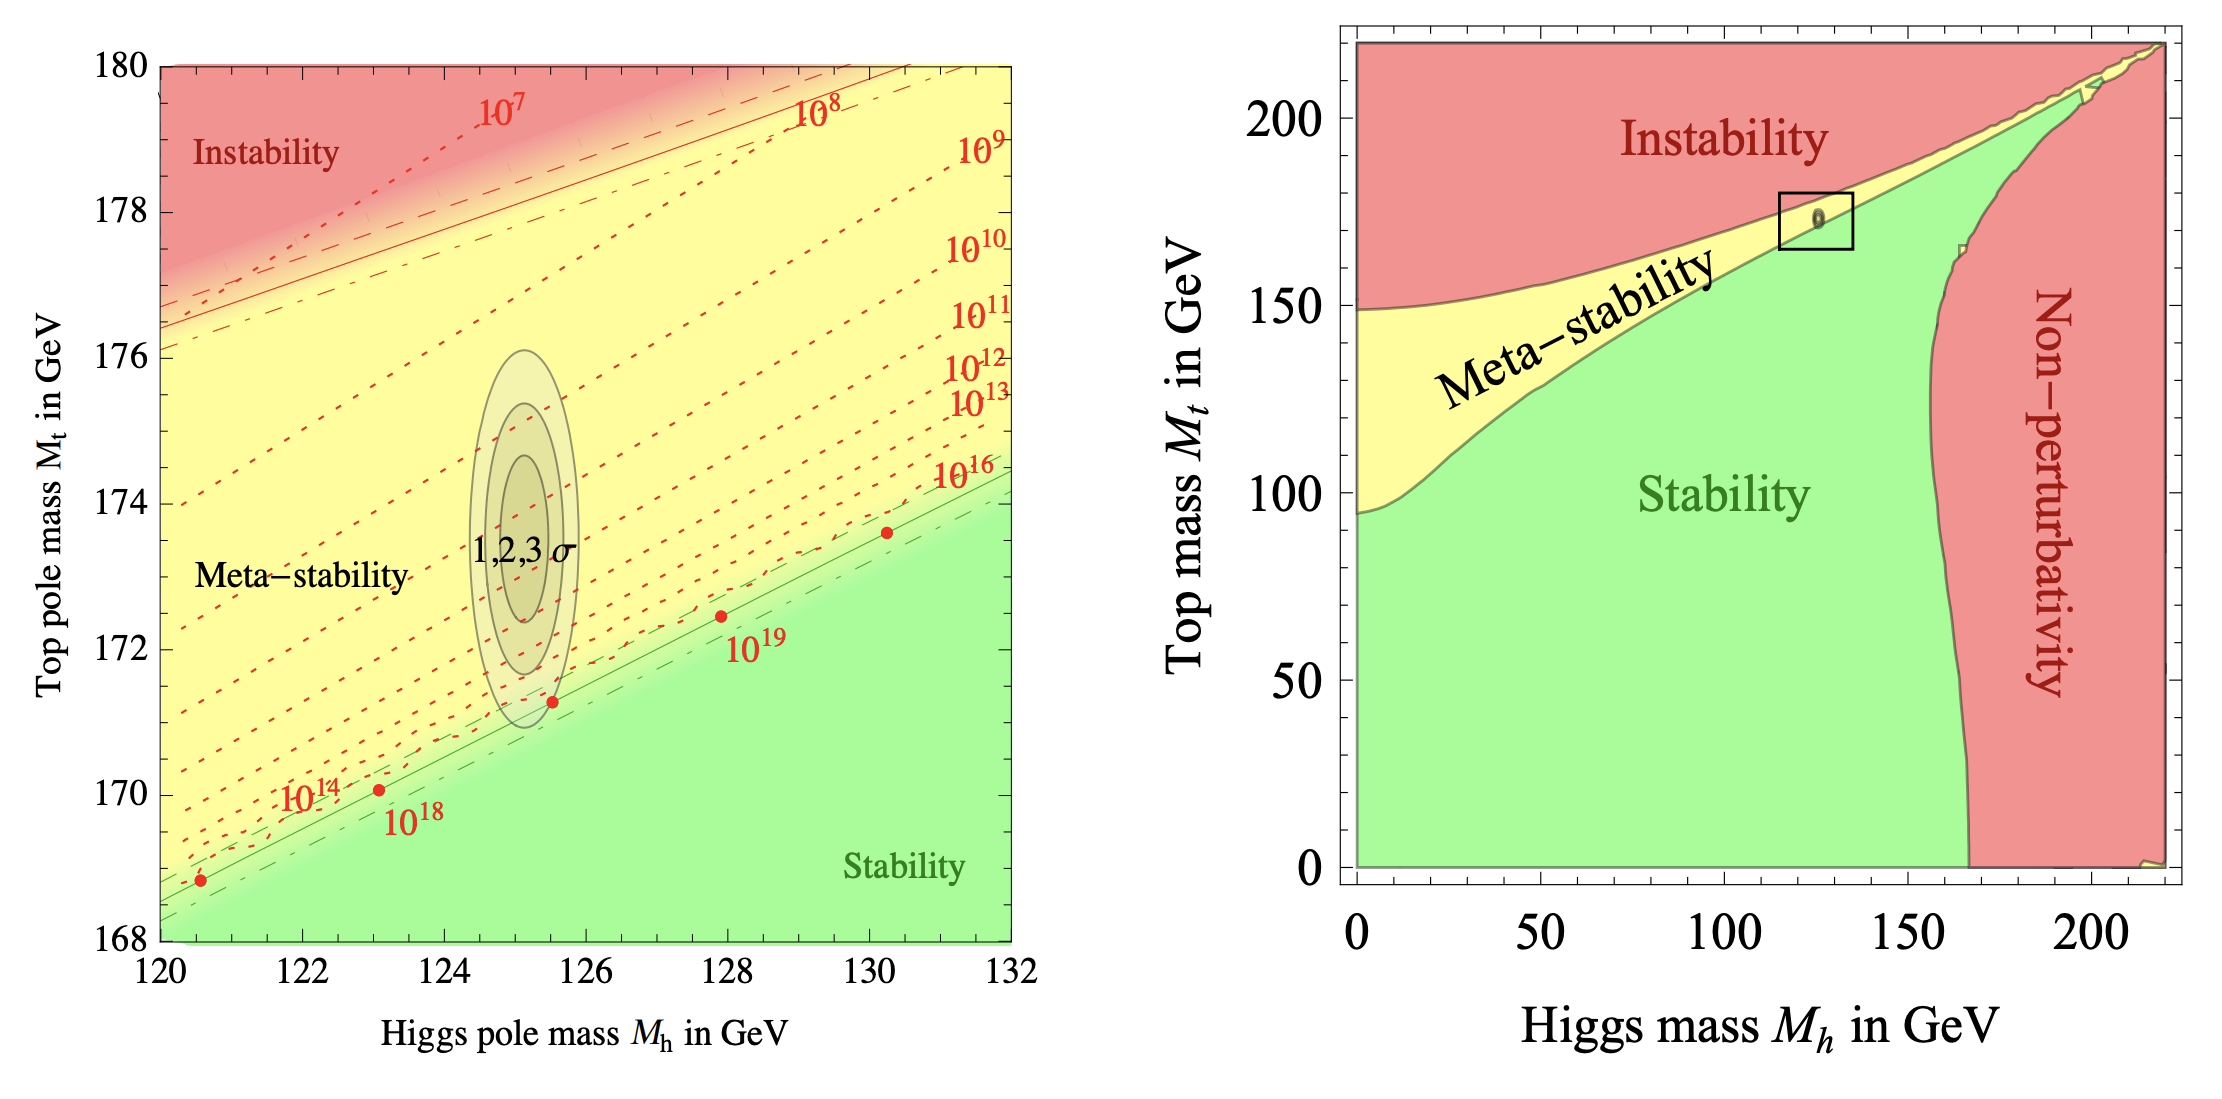
\includegraphics[width=0.6\textwidth]{Figures/stability.png}
\caption{Vacuum stability based on the Higgs-top mass, including constraints from collider experiments.}
\label{fig:stabilityPlot}
\end{figure}
 
A deeper understanding of the universal stability can only come from a more immediate knowledge of the electroweak symmetry breaking in the early universe. The nature of such a symmetry breaking directly connects to the global shape of the Higgs potential. By using the observation of di-Higgs events to constrain the Higgs self-coupling, we aim to provide the first probe of the global shape of the Higgs potential and address the question of the form of electroweak symmetry breaking in the early universe. This will greatly extend our understanding the fundamental vacuum which gives rise to the all-important Higgs field, and constrain its shape more precisely than ever before. This insight will allow humanity, for the first time, to address head-on the question of whether our  reality corresponds to a ``true” vacuum of a Higgs potential global minimum, or if indeed if our cosmological fate is more accurately described by a metastable,``false” vacuum existing in a non-global minimum of the Higgs potential (see Figure~\ref{fig:HiggsPotentials}). \\

\begin{figure}[!ht]
\centering
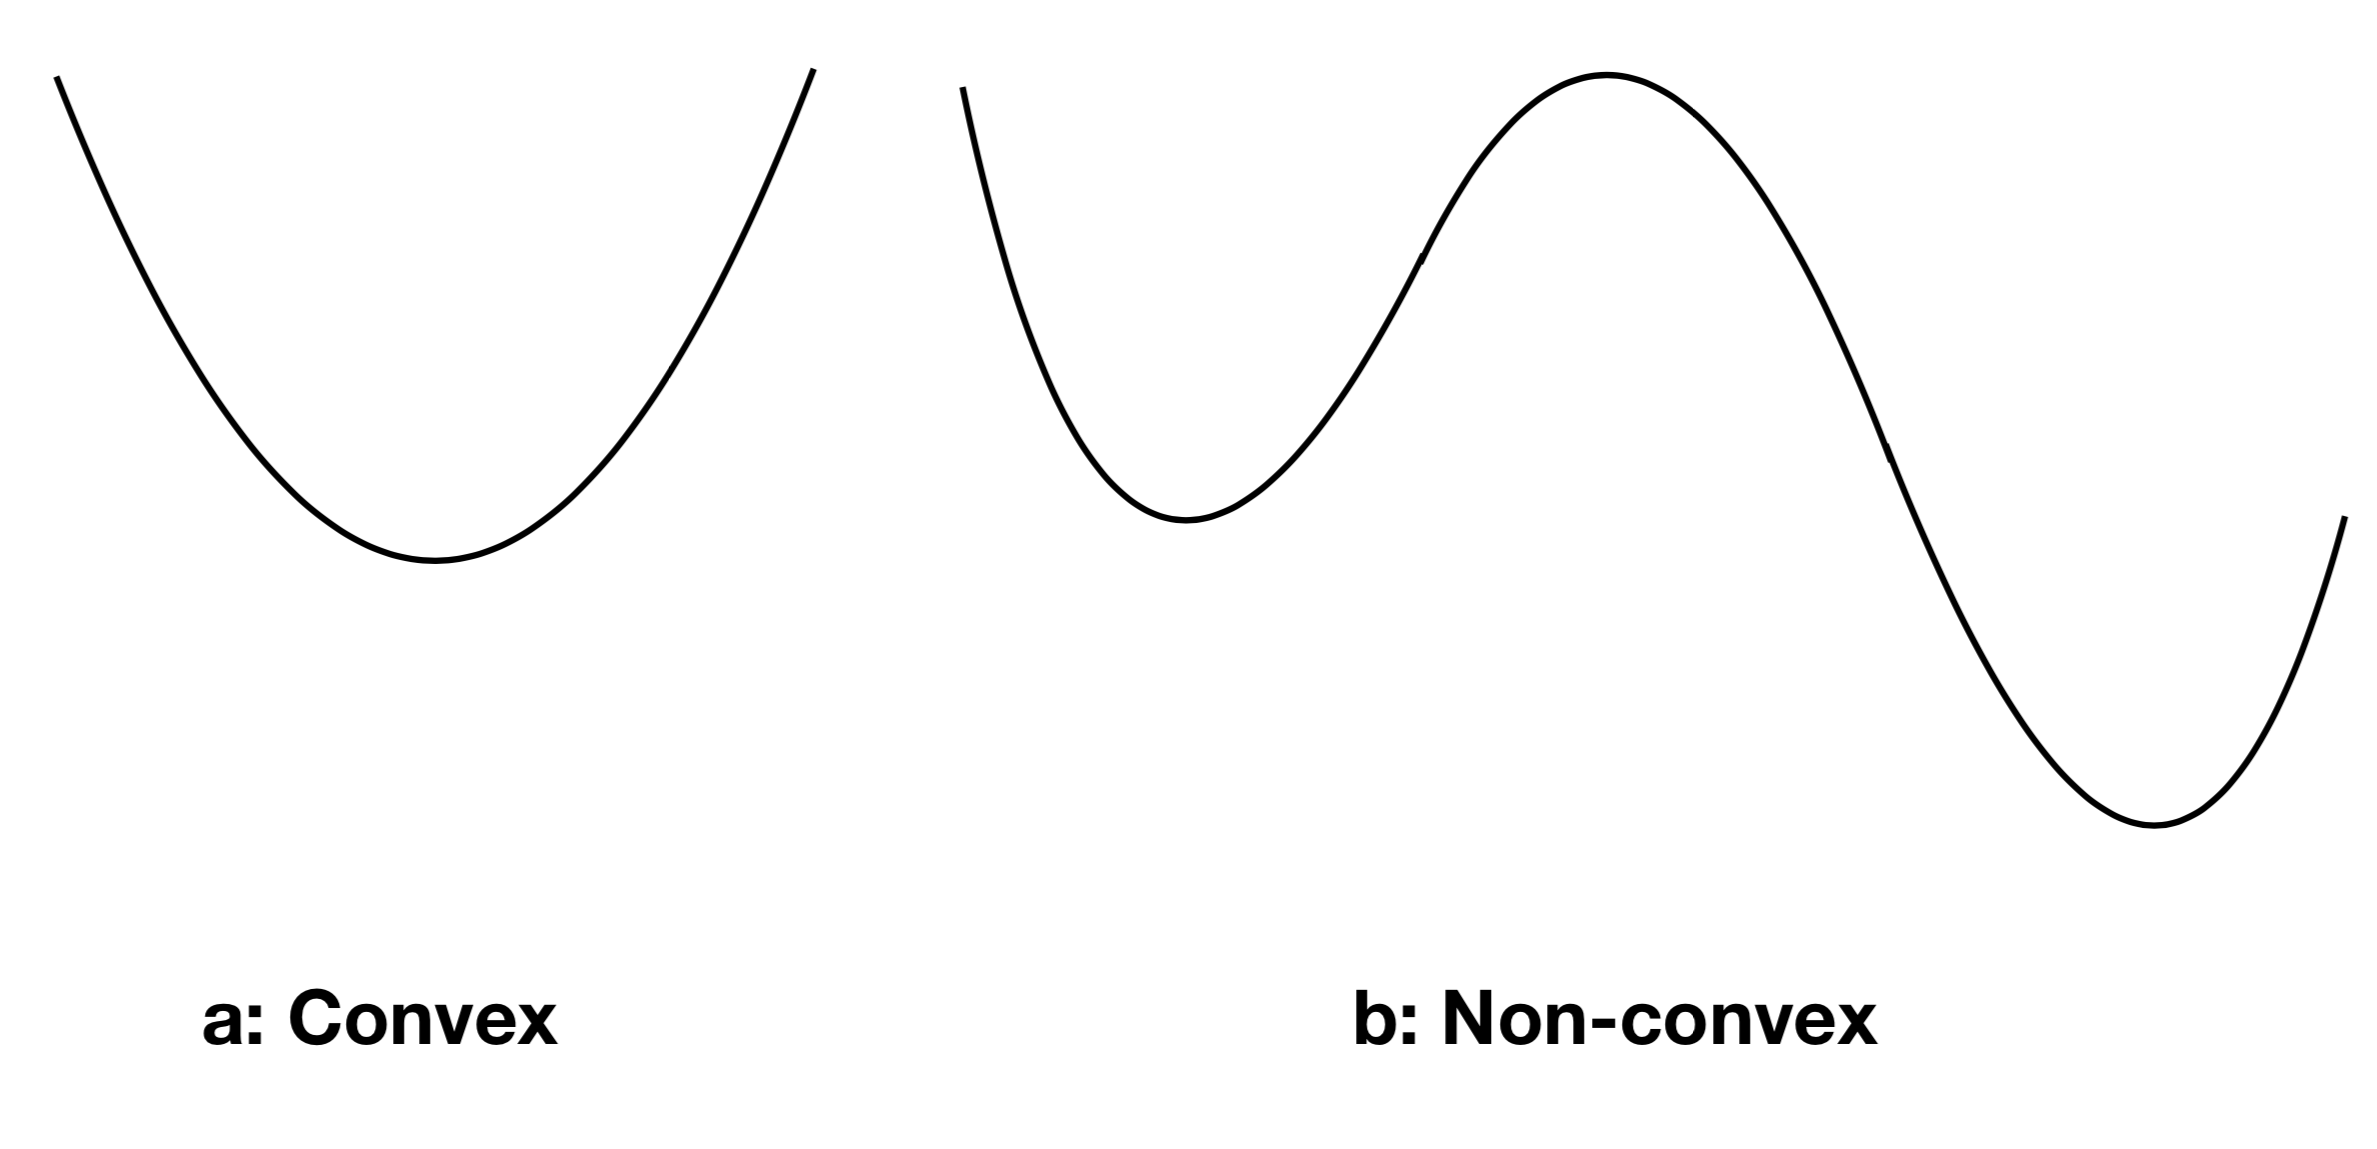
\includegraphics[width=0.6\textwidth]{Figures/HiggsPotentials.png}
\caption{Two possible Higgs potentials which describe could describe our universe. They have different global shapes and curvatures, and the local or global nature of their minima dictate the nature of the vacuum of our observable universe today. The potential in case $a$ is convex, and has a single global minimum corresponding to a true vacuum; case $b$ is non-convex, and has local and global minima, where the local minimum would correspond to a false vacuum.}
\label{fig:HiggsPotentials}
\end{figure}

Probing this question further: what can the nature of the Higgs potential tell us about its role in the cosmology of the early universe? We will seek to investigate two highly topical open problems in cosmology here: \\

\begin{itemize}
\item Open problem 1): What is nature of the Higgs boson during the period of universal inflation in the early universe. What was the physical process driving such an inflatory epoch? It could well be that the inflaton fields which generated this expected rapid expansion is deeply connected on the fundamental level to the Higgs field; both particles are scalars and both the physics of the Higgs and inflation are readily described as a phase-transition. Through probing the Higgs potential, we also seek to address this cosmological problem. \\
\item Open problem 2): How could the physics of the Higgs be influencing the production and observation of gravitational waves in our universe? Following the recent discovery of gravitational waves, we are seeking to understand if the Higgs self-coupling and potential can be used to constrain models of gravitational wave origin and production, and thus seek to establish the first connection between the physics of the very small and the physics of gravity; a concrete connection between these pillars of modern physics has thus far eluded experimentalists and theorists alike, but the Higgs might finally bring about the connection we are looking for. \\
\end{itemize}

\textit{We will need a paragraph here on the cosmology pheno outputs of the group at the time of submission of the grant}. \\

Sweden is an established leader in searches for di-Higgs final states, and this new project will unite the country's LHC searches across the $HH$ $\rightsarrow$ $b\bar{b}\gamma\gamma$, $b\bar{b}\tau\tau$, and multi-lepton final states to push the discovery boundaries of the Higgs self-coupling with LHC data and address these above open problems cosmological questions head-on. A combination of insights in cosmology and the deployment of the very latest machine learning techniques within the LHC analyses will guide and shape future developments towards the self-coupling discovery and Higgs potential measurements. Such results, gleaned through the combined effort of Sweden’s high-quality research in fundamental physics, will have a lasting effect on our understanding of the cosmology of our universe. \\

\subsection{Track 2: Di-Higgs as a Probe of Naturalness, Supersymmetry, Compositeness, and Beyond}

\begin{figure}[!ht]
\centering
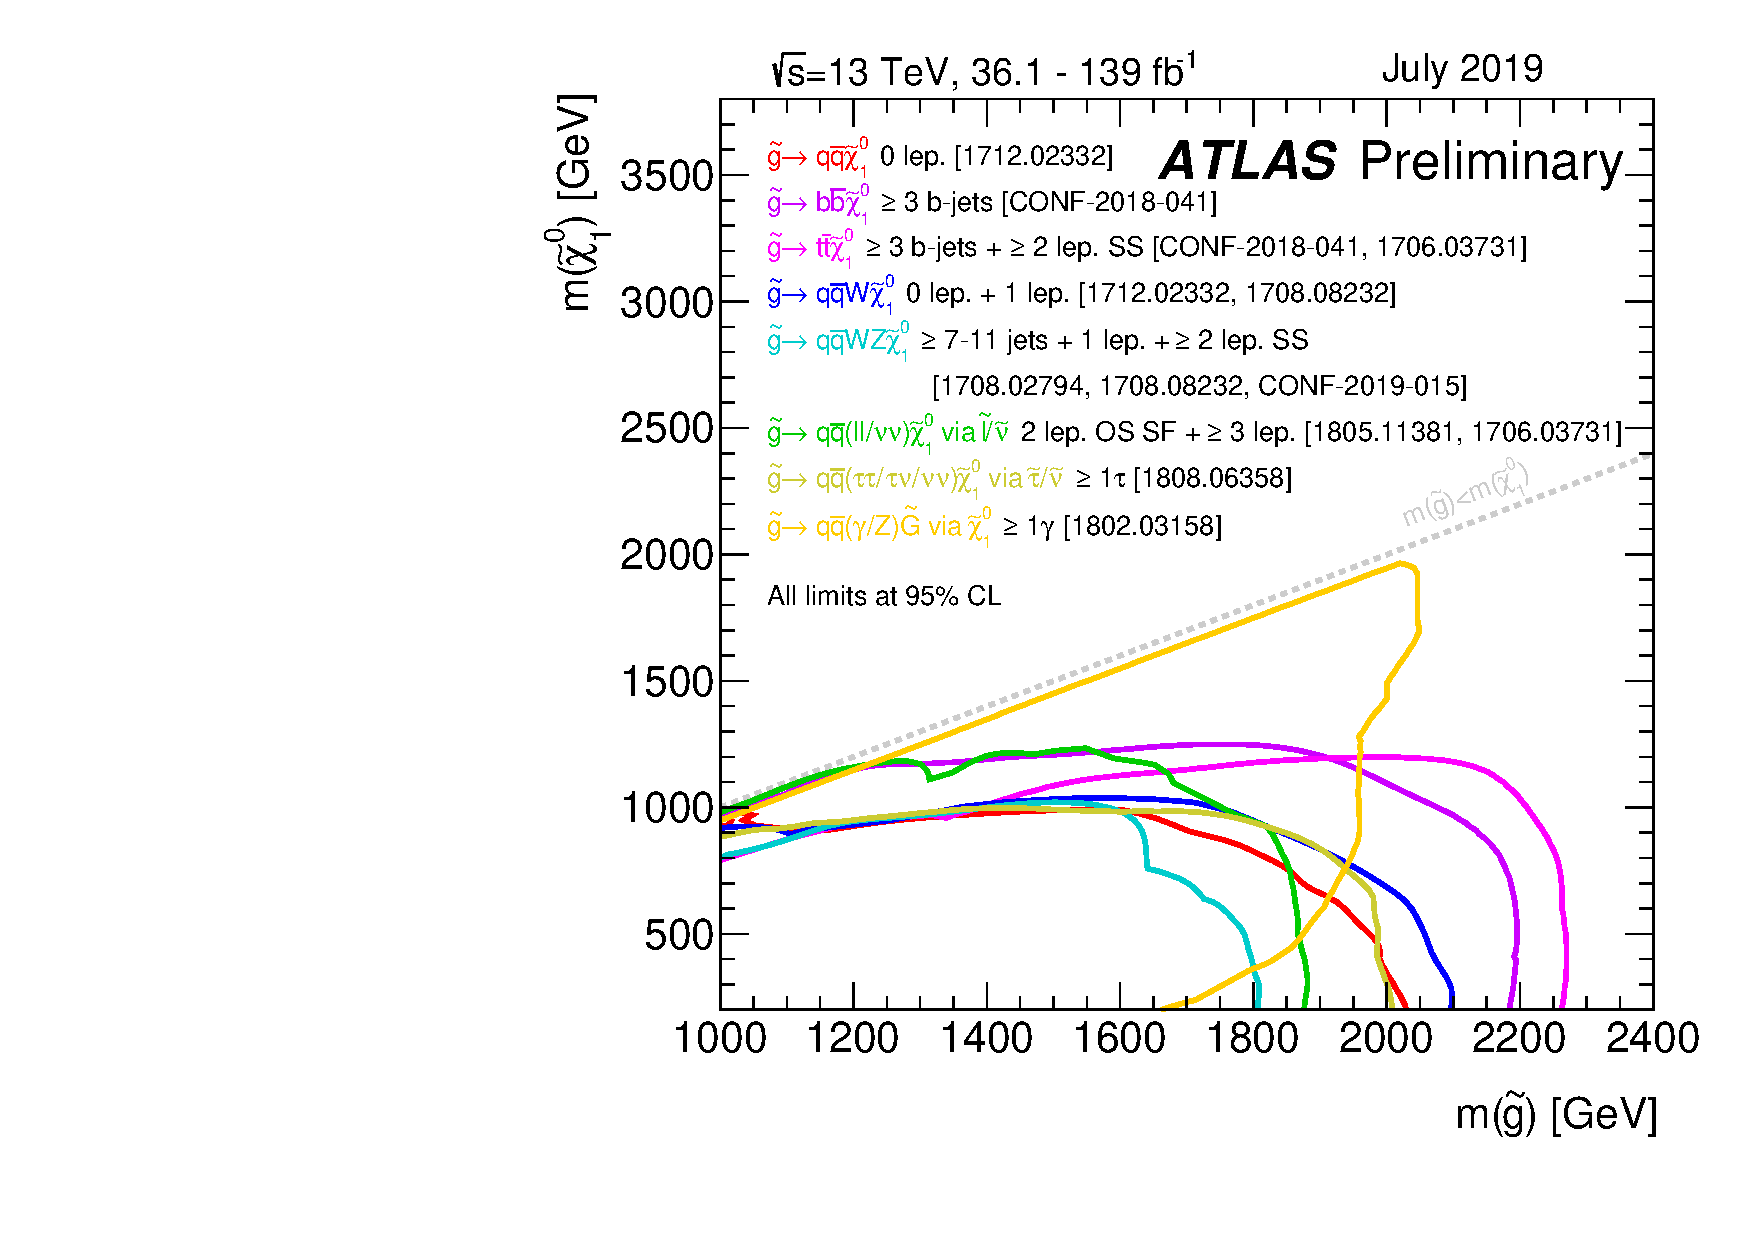
\includegraphics[width=0.5\textwidth]{Figures/summarySUSY}
\caption{Example constraints on gluino production in SUSY, with Run 2 ATLAS data.}
\label{fig:summarySUSY}
\end{figure}

\begin{figure}[!ht]
\centering
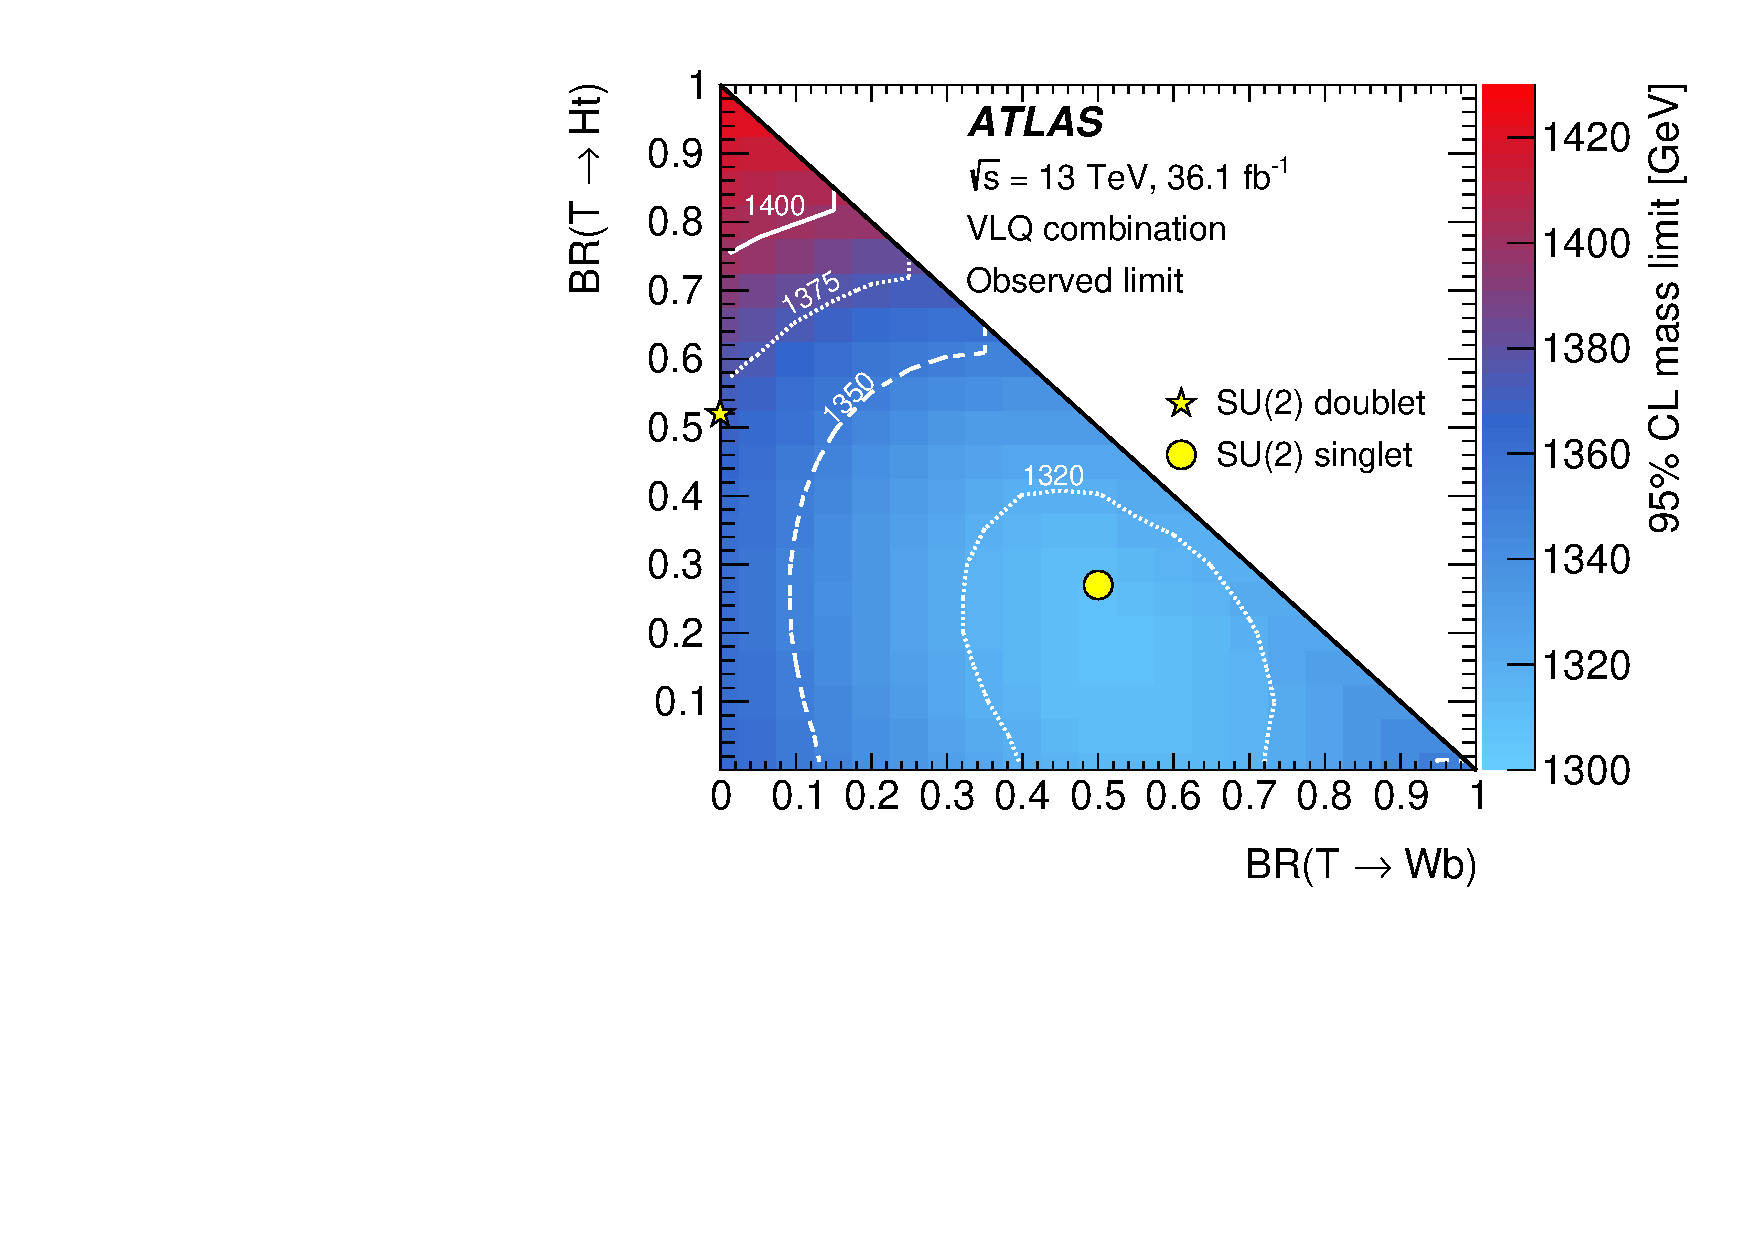
\includegraphics[width=0.5\textwidth]{Figures/summaryVLQs}
\caption{Example constraints on vector-like quark production, commonly predicted by Higgs Compositness models, with Run 2 ATLAS data.}
\label{fig:summaryVLQs}
\end{figure}

The Higgs self-coupling is also a crucial key for unlocking the door towards understanding the hierarchy problem, where the other best solutions to date — namely, Compositeness and SUSY [REF] — are becoming increasingly constrained by LHC data (see Figures~\ref{fig:summarySUSY} and~\ref{fig:summaryVLQs}). In (unbroken) SUSY, the Higgs self-coupling is the gauge coupling, so to measure or constrain it (through experimental searches or theoretical self-consistency) would provide an invaluable probe of supersymmetric physics scenarios. To further complement these studies, Compositeness comprises a key feature that there exists a strong correlation between the top Yukawa couplings and the Higgs self-coupling, since they can both be generated by the breaking of the pseudo-Nambu-Goldstone boson shift symmetry [REF]. Crucially, the Higgs self-coupling provides the ideal bridge between these two well-motivated theoretical extensions to the SM: Higgs pair-production captures both the quartic couplings Higgs-Higgs-stop-stop (Supersymmetry) and Higgs-Higgs-heavy-top-heavy-top (Compositeness). These are topologies which do not appear in the SM and which are intrinsically different in these two theoretical constructs, as in one case they are induced by top scalars (Supersymmetry) and in the other case by top fermions (Compositeness). It is therefore apparent that the nature of SUSY, Compositeness, and therefore the implications for naturalness and fine-tuning in our universe [REF], can be directly assessed through precision measurements of di-Higgs production at the LHC. Following our group's ongoing theoretical studies of SUSY and Compositeness contributions to di-Higgs production, we propose to conduct the first direct experimental probe of SUSY and Compositeness in di-Higgs production loops (see Figure~\ref{fig:diHiggsLoops}, and uniquely constrain these theoretical programmes in the di-Higgs sector. This proposal of probing naturalness with di-Higgs searches directly complements the ongoing SHiFT project [REF], which is seeking to address the nature of naturalness and fine-tuning through stop production at the LHC. Adding in the Higgs self-coupling to the picture will finally allow us to scan the veranda of phase-space where natural new physics might well be hiding. \\

\begin{figure}[!ht]
\centering
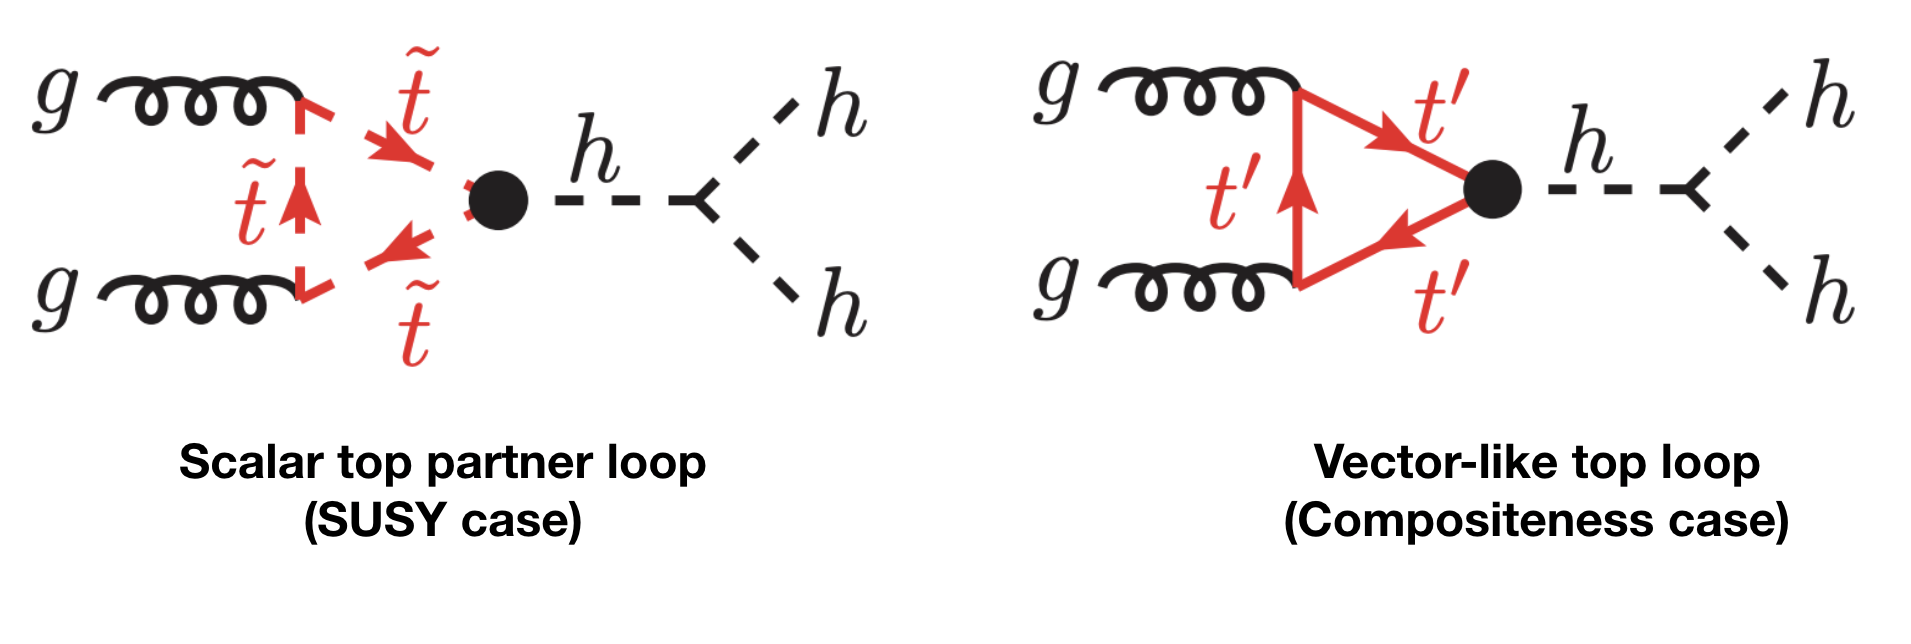
\includegraphics[width=0.6\textwidth]{Figures/diHiggsLoops}
\caption{Two possible scenarios where SUSY or Compositeness can directly enter di-Higgs production. Such physics is yet to be probed in LHC data.}
\label{fig:diHiggsLoops}
\end{figure}

To complement these model-inspired BSM studies, the model-independent approach of Effective Field Theory (EFT) will also be employed in the study of di-Higgs production. This complementary channel will ensure that a large chunk of the phase-space of new physics - from model-independent to more model-dependent production - can be probed and studied in the di-Higgs sector. We propose to provide the first constraint on the EFT extension of the SM in order to probe any new physics which could be manifest in that framework. The approach will be two-fold: first the EFT will be probed in a``local” way with Run-3 data, where the $\kappa_{\lambda}$ parameters will be constrained across all major di-Higgs channels ($ggH$/$ggt\bar{t}$/$gg$/$t\bar{t}$). Following on from this, longer-term goal will be the first ever ``global” EFT fit across both di-Higgs and single Higgs production modes with LHC data, providing the first combined constraint of single and di-Higgs couplings. This ``global fit'' approach will be the first of its kind, and will be the most complete model-independent constraint from the LHC on new physics in the Higgs sector. Never before will such a statistically challenging and rigorous combination of LHC results across single Higgs, di-Higgs, and electroweak physics have been studied to produce the most sensitive, high-profile probe of the nature of reality. \\

The third approach is the injection of novel new models which modify existing searches for di-Higgs production. We seek to modify the conventional di-Higgs discovery signature by developing analyses, driven by modern artificial intelligence and machine learning approaches, which can probe more general final states. The addition of a radiated hadronic jet to the final state is an ideal testing bed for using QCD as a probe of new physics which could otherwise not be observed in the conventional di-Higgs state (Figure~\ref{fig:addJet}); such approaches are entirely absent in all LHC searches, and will form the basis of a new line of high-profile analyses rolled out by the input of this grant. \\

\begin{figure}[!ht]
\centering
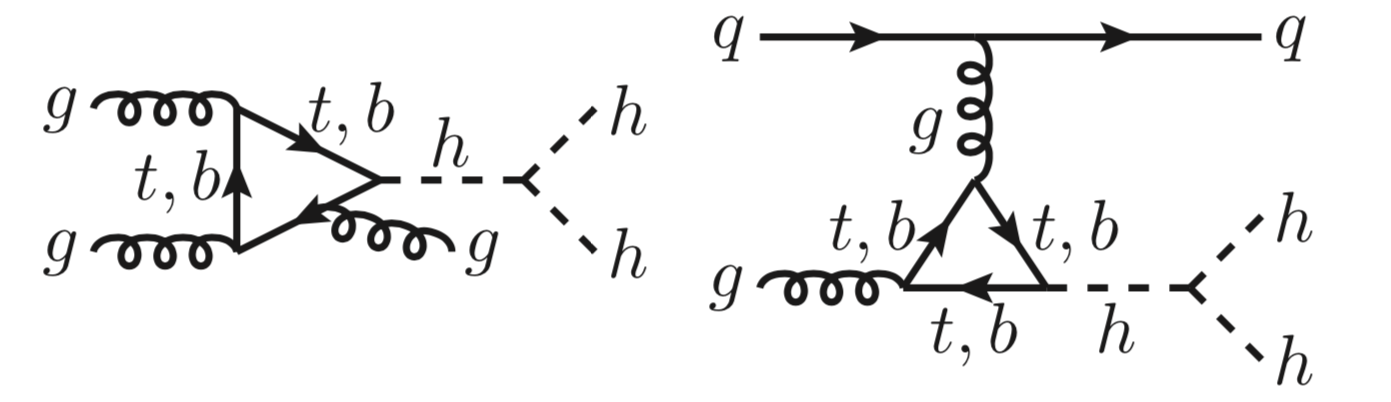
\includegraphics[width=0.6\textwidth]{Figures/addJet}
\caption{An example of a new final state being considered by this grant, whereby an additional hadronic jet is used to probe the new physics which could directly contribute to loops in di-Higgs production.}
\label{fig:addJet}
\end{figure}

\subsection{The Role of the Swedish Di-Higgs Working Group}

Throughout this project strong communication and collaboration between the LHC experimentalists and particle physics theorists will be paramount to any and all continued success. This communication effort has been realised in the founding of the Swedish Di-Higgs Working Group, a forum for communication between experimentalists at Stockholm, KTH, Lund, and Uppsala, as well as theorists in Uppsala and Lund. One of the major deliverables of this new group is the publication of several new BSM-inspired physics papers which can be used to propose new approaches to probing the direct production of new matter in di-Higgs final states at the LHC. Establishing these joint publications between experimentalists and theorists generates a natural symbiosis in which the di-Higgs searches at ATLAS can be directly interpreted within the theory community. The presence of this exciting collaboration also further strengthens Sweden's position as an international powerhouse of Higgs physics. Furthermore, a second major goal of this collaboration will be the study of new models, beyond SUSY, Compositeness, and convention heavy resonances, which could shed light on the nature of the eventual observation of the di-Higgs final state and therefore reveal the deepest secrets of the fundamental building blocks of our universe, as well as its underlying cosmology. This ongoing theoretical work has already been realised in several ongoing studies and publications from the Swedish Di-Higgs Working Group $-$ please see $\textit{and here we need to rattle off our ongoing and published papers as a group, in time for the grant submission}$. This group is also dedicated to investigating the known shortcoming of current experimental and theoretical understanding of the di-Higgs sector (as realised in the group's recent white paper $-$ please see $\textit{comment on white paper}$). \\

The complete landscape of the Swedish Di-Higgs Working Group and this project, including connections between the major tracks, is displayed schematically in Figure~\ref{fig:connections}. \\

\begin{figure}[!ht]
\centering
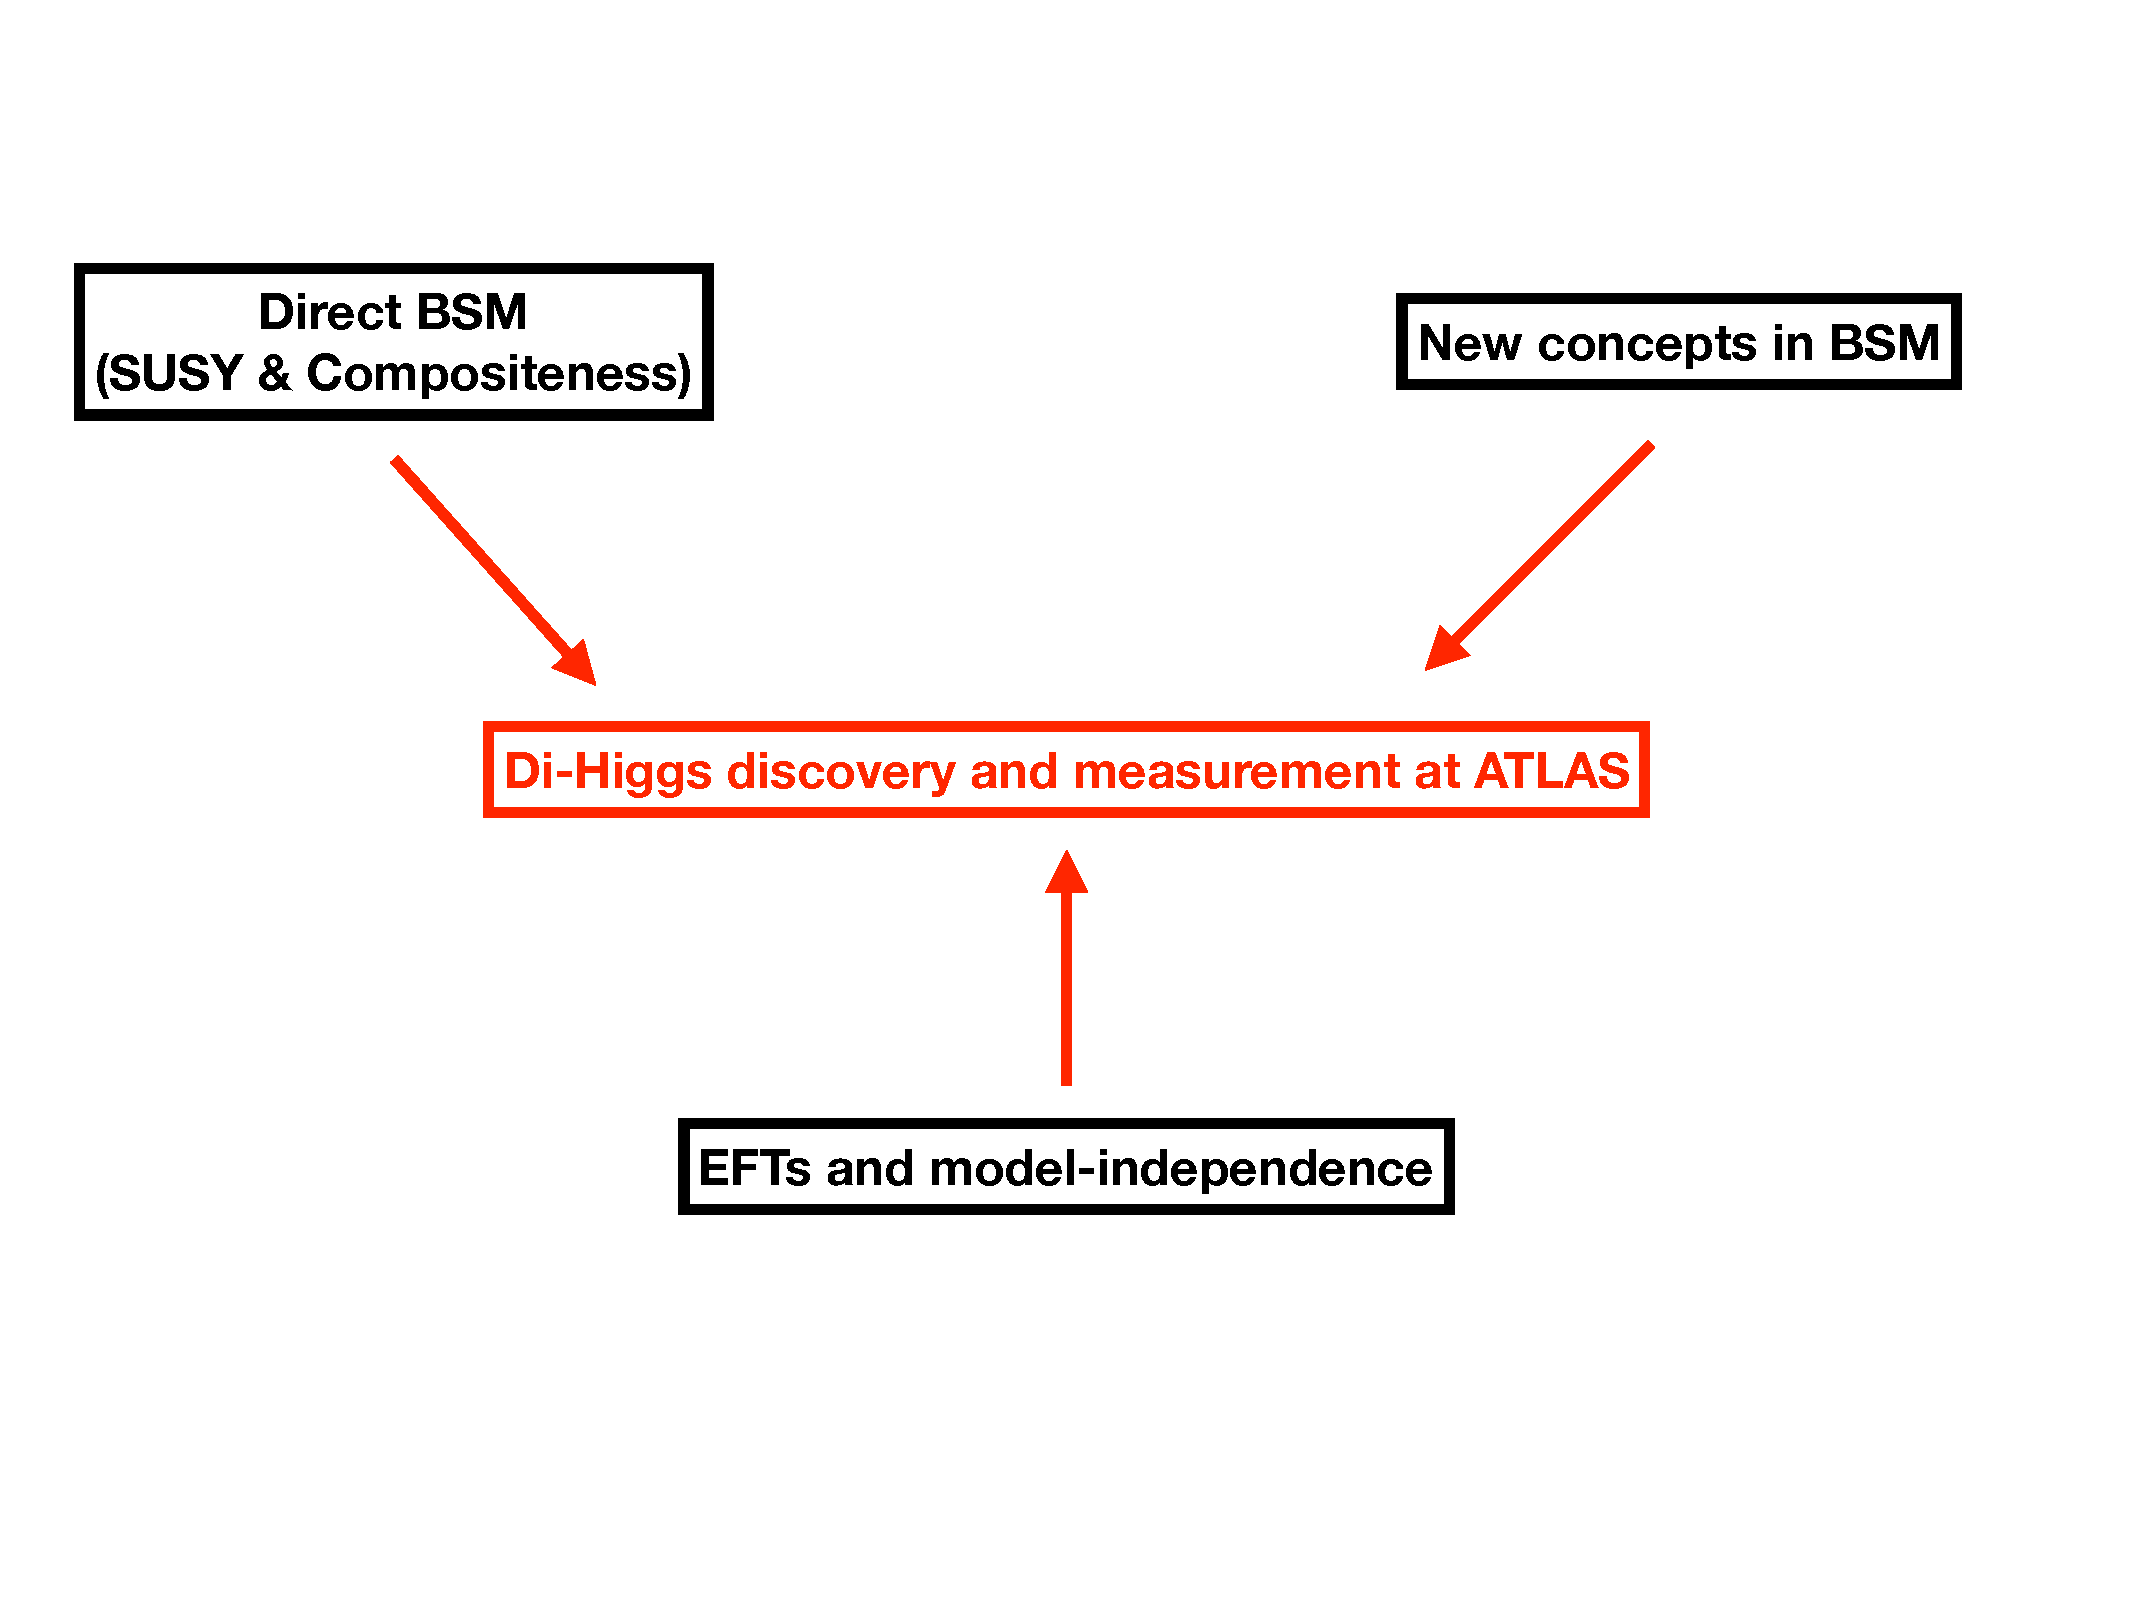
\includegraphics[width=0.75\textwidth]{Figures/ConnectionsAcrossGrant}
\caption{A schematic illustrating the connections between different aspects of BSM searches, and di-Higgs production. Major connections which this project will establish are (i) direct BSM (SUSY, Compositeness); (ii) model-independent BSM/EFTs; and (iii) new concepts in BSM. All three approaches will be pursued by the Swedish Di-Higgs Working Group as part of this proposed grant. }
\label{fig:connections}
\end{figure}

\section{Deliverables and Timescales}

\textit{Let's try and finalise this section at the meeting, and come up with a complete timeline.}\\

This project will complement the existing SHiFT grant, by further extending the question of addressing naturalness and beyond SM physics through direct measurements of the Higgs boson, in contrast to direct measurements of stop production at the LHC which is the primary focus of SHiFT. TThe intended funding for this project is expected to begin as SHiFT draws to a close. This provides an organic and efficient bridge, such that we can learn from the world-leading research of the SHiFT grant, and use that projects important results to complement nicely the search for new physics through di-Higgs discovery at the LHC. As already mentioned, the work within this project will build from the output of the Swedish Di-Higgs Working Group, and this team of collaborators provides a natural forum in which to lead the projects and results within this grant.  The timeline and deliverables leading up to the proposed start of funding, and during the funding period, are summarised in Figure~\ref{fig:timeline}. 

\begin{figure}[!ht]
\centering
\includegraphics[width=0.3\textwidth]{Figures/}
\caption{A schematic of the timeline for the project, including the early results before publication. TODO: construct schematic based on discussions at the meeting.}
\label{fig:timeline}
\end{figure}

\begin{itemize}
\item A series of publications, led by high-quality and world-leading Swedish researchers, in to di-Higgs final states by the end of Run 3 of the LHC (2024).
\item R&D leading up to the first statistically significant Higgs self-coupling measurement and test of universal cosmology at the High-Luminosity LHC (2026). 
\item The rapid expansion of the Swedish Di-Higgs Working Group and the recruitment of several PhD and postdoctoral research fellows between 2021 (intended start of the grant) and 2024. 
\item The publication of Run 3 summary papers across the di-Higgs $b\bar{b}\gamma\gamma$, $b\bar{b}\tau\tau$, multi-lepton channels, and the combined limit LHC papers by 2024.
\item The development of non-minimal theoretical models beyond SUSY and Compositeness, in the period 2021-2024, with deployment of those models in di-Higgs searches using Run 3 data (2024).
\item The deployment of these new BSM models at the HL-LHC (2026).
\item The first complete treatment of EFTs in a global fit including di-Higgs analysis results, with Run 3 of the LHC. This will be a series of papers between 2023 and 2026. 
\item A series of national workshops, lead by the Swedish Di-Higgs Working Group, pooling  expertise across Sweden in theoretical and experimental physics, with the aim of further generating research output from the group, such that the highest quality results are prepared and ready by the start of the HL-LHC (2021-2026). These workshops will aim to bring together experts from the communities of particle physics and cosmology, a unique combination of the two disciplines, in order to tackle di-Higgs physics from a truly global angle, and will further cement Sweden's global reputation in Higgs physics. 
\end{itemize}

\end{document}


